\begin{SCn}
\scnheader{Менеджер многократно используемых компонентов ostis-систем}
\begin{scnrelfromlist}{ключевой знак}
	\scnitem{Реализация менеджера многократно используемых компонентов ostis-систем}
	\scnitem{Пример структуры хранилища адресов спецификаций компонентов}
\end{scnrelfromlist}
\end{SCn}

\begin{SCn}
\begin{scnrelfromlist}{ключевое понятие}
	\scnitem{менеджер многократно используемых компонентов ostis-систем}
\end{scnrelfromlist}
\end{SCn}

\begin{SCn}
\begin{scnrelfromlist}{ключевое знание}
	\scnitem{Минимальные функциональные возможности менеджера компонентов}
	\scnitem{Расширенные функциональные возможности менеджера компонентов}
\end{scnrelfromlist}
\end{SCn}

\bigskip

\textbf{\textit{менеджер многократно используемых компонентов ostis-систем}} --- подсистема ostis-системы, с помощью которой происходит взаимодействие с библиотекой компонентов ostis-систем.

\begin{SCn}
\scnheader{менеджер многократно используемых компонентов ostis-систем}
\scnsubset{встраиваемая ostis-система}
\scnsubset{платформенно-зависимый многократно используемый компонент ostis-систем}
\scnidtftext{часто используемый sc-идентификатор}{менеджер многократно используемых компонентов}
\scnidtftext{часто используемый sc-идентификатор}{менеджер компонентов}
\begin{scnrelfromset}{обобщенная декомпозиция}
	\scnitem{база знаний менеджера многократно используемых компонентов ostis-систем}
	\scnitem{решатель задач менеджера многократно используемых компонентов ostis-систем}
	\scnitem{интерфейс менеджера многократно используемых компонентов ostis-систем}
\end{scnrelfromset}
\scnhaselement{Реализация менеджера многократно используемых компонентов ostis-систем}
\begin{scnindent}
	\scntext{адрес компонента}{https://github.com/ostis-ai/sc-component-manager}
\end{scnindent}
\end{SCn}

\textbf{\textit{база знаний менеджера многократно используемых компонентов ostis-систем}} содержит все те знания, которые необходимы для установки многократно используемого компонента в дочернюю ostis-систему. К таким знаниям относятся знания о спецификации многократно используемых компонентов, методы установки компонентов, знание о библиотеках ostis-систем, с которыми происходит взаимодействие, \textit{Классификация компонентов} и другие. \textbf{\textit{решатель задач менеджера многократно используемых компонентов ostis-систем}} взаимодействует с \textit{библиотекой ostis-систем} и позволяет установить и интегрировать многократно используемые компоненты в дочернюю ostis-систему, также выполнять поиск, обновление, публикацию, удаление компонентов и другие операции с ними. \textbf{\textit{интерфейс менеджера многократно используемых компонентов ostis-систем}} обеспечивает удобное для пользователя и других систем использование менеджера компонентов.

\textit{решатель задач менеджера многократно используемых компонентов ostis-систем} как минимум должен обеспечивать следующие функциональные возможности:

\begin{SCn}
\scnheader{менеджер многократно используемых компонентов ostis-систем}
\scnrelfrom{минимальные функциональные возможности}{Минимальные функциональные возможности менеджера компонентов}
\begin{scnindent}
\begin{scneqtoset}
	\scnfileitem{\textbf{Поиск многократно используемых компонентов ostis-систем.} Множество возможных критериев поиска соответствует спецификации многократно используемых компонентов. Такими критериями могут быть классы компонента, его авторы, идентификатор, фрагмент примечания, назначение, принадлежность какой-либо предметной области, вид знаний компонента и другие.}
	\scnfileitem{\textbf{Установка многократно используемого компонента ostis-систем.} Установка многократно используемого компонента происходит вне зависимости от типологии, способа установки и местоположения компонента. Необходимое условие для возможности установки многократно используемого компонента --- наличие \textbf{\textit{спецификации многократно используемого компонента ostis-систем}}. Перед установкой многократно используемого компонента в дочернюю систему необходимо установить все зависимые компоненты. Также для платформенно-зависимых компонентов может быть необходимо установить иные зависимости, которые не являются компонентами какой-либо библиотеки ostis-систем. После успешной установки компонента в базе знаний дочерней системы генерируется информационная конструкция, обозначающая факт установки компонента в систему с помощью отношения \textit{установленные компоненты*}.}
	\scnfileitem{\textbf{Добавление и удаление отслеживаемых менеджером компонентов библиотек.} Менеджер компонентов содержит информацию о множестве источников для установки компонентов, перечень которых можно дополнять. По умолчанию менеджер компонентов отслеживает \textit{Библиотеку Метасистемы OSTIS}, однако можно создавать и добавлять дополнительные библиотеки ostis-систем.}
\end{scneqtoset}
\end{scnindent}
\end{SCn}

Исходя из указанных минимальных функциональных возможностей \textit{решатель задач менеджера многократно используемых компонентов ostis-систем} представляет собой следующую иерархию абстрактных sc-агентов:

\begin{SCn}
	\scnheader{решатель задач менеджера многократно используемых компонентов ostis-систем}
	\begin{scnrelfromset}{декомпозиция абстрактного sc-агента}
		\scnitem{Абстрактный sc-агент поиска многократно используемых компонентов ostis-систем}
		\scnitem{Абстрактный sc-агент установки многократно используемых компонентов ostis-систем}
		\scnitem{Абстрактный sc-агент управления отслеживаемых менеджером компонентов библиотек}
		\begin{scnindent}
			\begin{scnrelfromset}{декомпозиция абстрактного sc-агента}
				\scnitem{Абстрактный sc-агент добавления отслеживаемой менеджером компонентов библиотеки}
				\scnitem{Абстрактный sc-агент удаления отслеживаемой менеджером компонентов библиотеки}
			\end{scnrelfromset}
		\end{scnindent}
	\end{scnrelfromset}
\end{SCn}

Используя минимальные функциональные возможности менеджер компонентов может установить компоненты, которые будут расширять его же функционал. Компоненты, реализующие расширенный функционал менеджера компонентов являются частью \textit{Библиотеки Метасистемы OSTIS}. К расширенному функционалу относится:

\begin{SCn}
\scnheader{менеджер многократно используемых компонентов ostis-систем}
\scnrelfrom{расширенные функциональные возможности}{Расширенные функциональные возможности менеджера компонентов}
\begin{scnindent}
	\begin{scneqtoset}
		\scnfileitem{\textbf{Спецификация} многократно используемого компонента ostis-систем. Менеджер компонентов позволяет специфицировать компоненты, входящие в состав библиотеки ostis-систем, а также специфицировать новые создаваемые компоненты, которые будут публиковаться в библиотеку ostis-систем. При этом спецификация может происходить как автоматически, так и вручную. Например, менеджер компонентов может обновить спецификацию используемого компонента в соответствии с тем, в какие новые ostis-системы его установили, обновить спецификацию авторства компонента при его редактировании в библиотеке ostis-систем, спецификацию ошибок, выявленных в процессе эксплуатации компонента и так далее.}
		\scnfileitem{\textbf{Формирование} многократно используемого компонента ostis-систем по шаблону с заданными параметрами. При установке шаблона многократно используемого компонента ostis-систем менеджер компонентов позволяет сформировать по нему конкретный компонент. Для этого пользователю предлагается определить значения всех sc-переменных в шаблоне для формирования конкретного компонента из некоторой предметной области. Например, для формирования многократно используемого компонента баз знаний, представляющего собой семантическую окрестность некоторого отношения, нужно определить значения всех переменных, кроме переменной, являющейся ключевым sc-элементом данной структуры.}
		\bigskip
		\bigskip
		\scnfileitem{\textbf{Публикация} многократно используемого компонента ostis-систем в библиотеку ostis-систем. При публикации компонента в библиотеку ostis-систем происходит верификация на основе спецификации компонента. Публикация компонента может сопровождаться сборкой неатомарного компонента из существующих атомарных. Также существует возможность обновления версии опубликованного компонента сообществом его разработчиков.}
		\scnfileitem{\textbf{Обновление} установленного многократно используемого компонента ostis-систем.}
		\scnfileitem{\textbf{Удаление} установленного многократно используемого компонента. Как и в случае установки после удаления многократно используемого компонента из ostis-системы в базе знаний системы устанавливается факт удаления компонента. Эта информация является важной частью \underline{истории эксплуатации} ostis-системы.}
		\scnfileitem{\textbf{Редактирование} многократно используемого компонента в библиотеке ostis-систем.}
		\scnfileitem{\textbf{Сравнение} многократно используемых компонентов ostis-систем.}
	\end{scneqtoset}
\end{scnindent}
\end{SCn}

Для того, чтобы создать новую ostis-систему "с нуля"{}, используя \textit{ostis-платформу}, необходимо установить некоторый \textit{Программный вариант реализации ostis-платформы} с помощью сторонних средств. Такими средствами могут быть (1) хранилища исходного кода платформы, например, облачные хранилища, такие как GitHub репозиторий, с соответствующим набором инструкций по установке платформы или (2) средства установки заранее скомпилированной программной реализации платформы, например, средство установки программного обеспечения apt. Далее установка многократно используемых компонентов в ostis-систему (независимо от типа компонентов) осуществляется с помощью менеджера компонентов. При установке платформенно-зависимых компонентов менеджер компонентов должен управлять соответствующими средствами сборки таких компонентов (CMake, Ninja, npm, grunt и другие).

Компонент находится в некотором хранилище --- (1) \textit{библиотеке компонентов ostis-систем} или (2) в виде файлов в некотором облачном хранилище. В случае, когда компонент хранится в библиотеке, для его установки менеджер компонентов копирует все sc-элементы, которые представляют собой компонент, в дочернюю ostis-систему. В случае, когда компонент хранится в виде файлов в облачном хранилище, менеджер компонентов скачивает файлы компонента и устанавливает их в соответствии со спецификацией. Адреса хранилищ спецификаций компонентов должны храниться в базе знаний менеджера компонентов, чтобы иметь доступ к спецификациям компонентов для их последующего использования (поиска, установки и так далее). На рисунке \textit{\ref{fig:specification_storage_addresses}} приведен пример фрагмента базы знаний менеджера компонентов, который описывает то, где хранятся спецификации компонентов, доступных для установки. Такое хранилище представляет собой множество, состоящее из двух множеств: (1) множество адресов спецификаций компонентов и (2) множество адресов спецификаций других хранилищ. Таким образом, образуется древовидная структура в соответствии с иерархией материнских ostis-систем и соответствующих им библиотек.

\begin{figure}[h]
	\caption{SCg-текст. Пример структуры хранилища адресов спецификаций компонентов}
	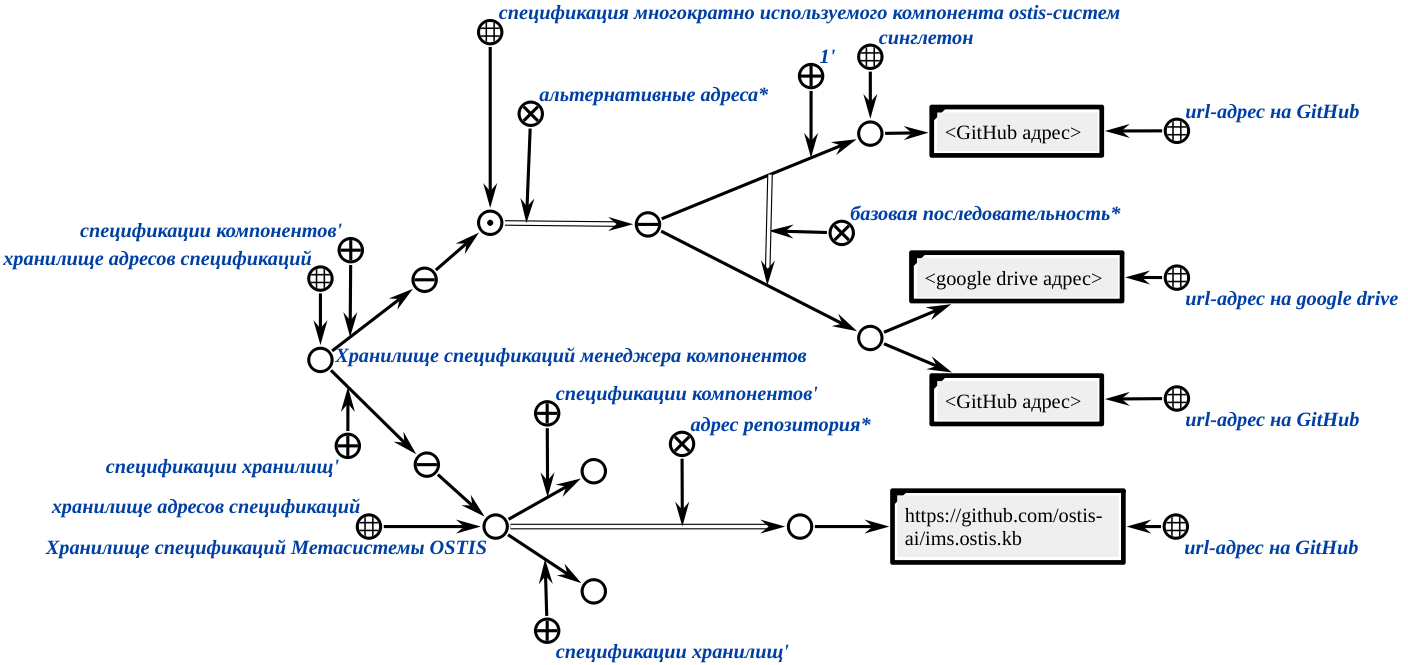
\includegraphics[scale=0.4]{images/specification_storage_addresses.png}
	\label{fig:specification_storage_addresses}
\end{figure}

Если указать адрес корня дерева хранилищ адресов спецификаций, то менеджер компонентов получает доступ ко всем спецификациям дочерних хранилищ. При обработке такого дерева спецификаций менеджер компонентов погружает в sc-память спецификации компонентов, доступных для установки, однако не сами эти компоненты.

\textit{менеджер многократно используемых компонентов ostis-систем} является \underline{необязательной} подсистемой \textit{ostis-платформы}. Однако система, имеющая менеджер компонентов, может устанавливать компоненты не только сама в себя, но и в другие системы при наличии доступа. Таким образом, одна система может заменить \textit{ostis-платформу} другой системы, оставив при этом \textit{sc-модель кибернетической системы}. Таким же образом некоторая ostis-система может порождать другие ostis-системы, используя компонентный подход.

Включение компонента в \textit{дочернюю ostis-систему} в общем случае состоит из следующих этапов:
\begin{itemize}
	\item поиск подходящего компонента во множестве доступных библиотек;
	\item выделение компонента в виде, удобном для транспортировки в дочернюю ostis-систему с указанием версии и модификации при необходимости (например, выбор доступного хранилища компонента, выбор оптимального варианта реализации компонента с учетом состава дочерней системы);
	\item установка многократно используемого компонента и его зависимостей (с указанием версии и модификации при необходимости);
	\item интеграция компонента в дочернюю систему;
	\item поиск и устранение ошибок и противоречий в дочерней системе.
\end{itemize}

Данный процесс с точки зрения пользователя не зависит от типа компонента и особенностей его реализации.
